%!TEX TS-program = xelatex
%!TEX encoding = UTF-8 Unicode
\documentclass[12pt,a4paper]{article}
\usepackage{geometry} % 設定邊界
\geometry{
  top=1in,
  inner=1in,
  outer=1in,
  bottom=1in,
  headheight=3ex,
  headsep=2ex
}
\usepackage{fontspec} % 允許設定字體
\usepackage{xeCJK} % 分開設置中英文字型
\usepackage{url} % 使用url
\setCJKmainfont{LiHei Pro} % 設定中文字型
\setmainfont{Georgia} % 設定英文字型
\setromanfont{Georgia} % 字型
\setmonofont{Courier New}
\linespread{1.2}\selectfont % 行距
\XeTeXlinebreaklocale "zh" % 針對中文自動換行
\XeTeXlinebreakskip = 0pt plus 1pt % 字與字之間加入0pt至1pt的間距,確保左右對整齊
\parindent 0em % 段落縮進
\setlength{\parskip}{20pt} % 段落之間的距離

\title{\huge 影像處理 Assignment1 - 合併影像} % 設置標題,使用巨大字體
\author{姓名:吳嘉偉\quad 學號:5105056013\quad 日期:2017/12/10} % 設置作者
\date{} % 設置日期
\usepackage{titling}
\setlength{\droptitle}{-8em} % 將標題移動至頁面的上面
\usepackage{listings}

\begin{document}

\clearpage

\maketitle % 顯示標題

\section{合併步驟}

\subsection{三點座標}

{
\fontsize{14pt}{10pt} % 字型大小14pt,字行間距20pt
\selectfont % 生效
找出兩張圖對應的三點座標,此三點圍成的面積越大越好
\begin{figure}[ht]
\centering
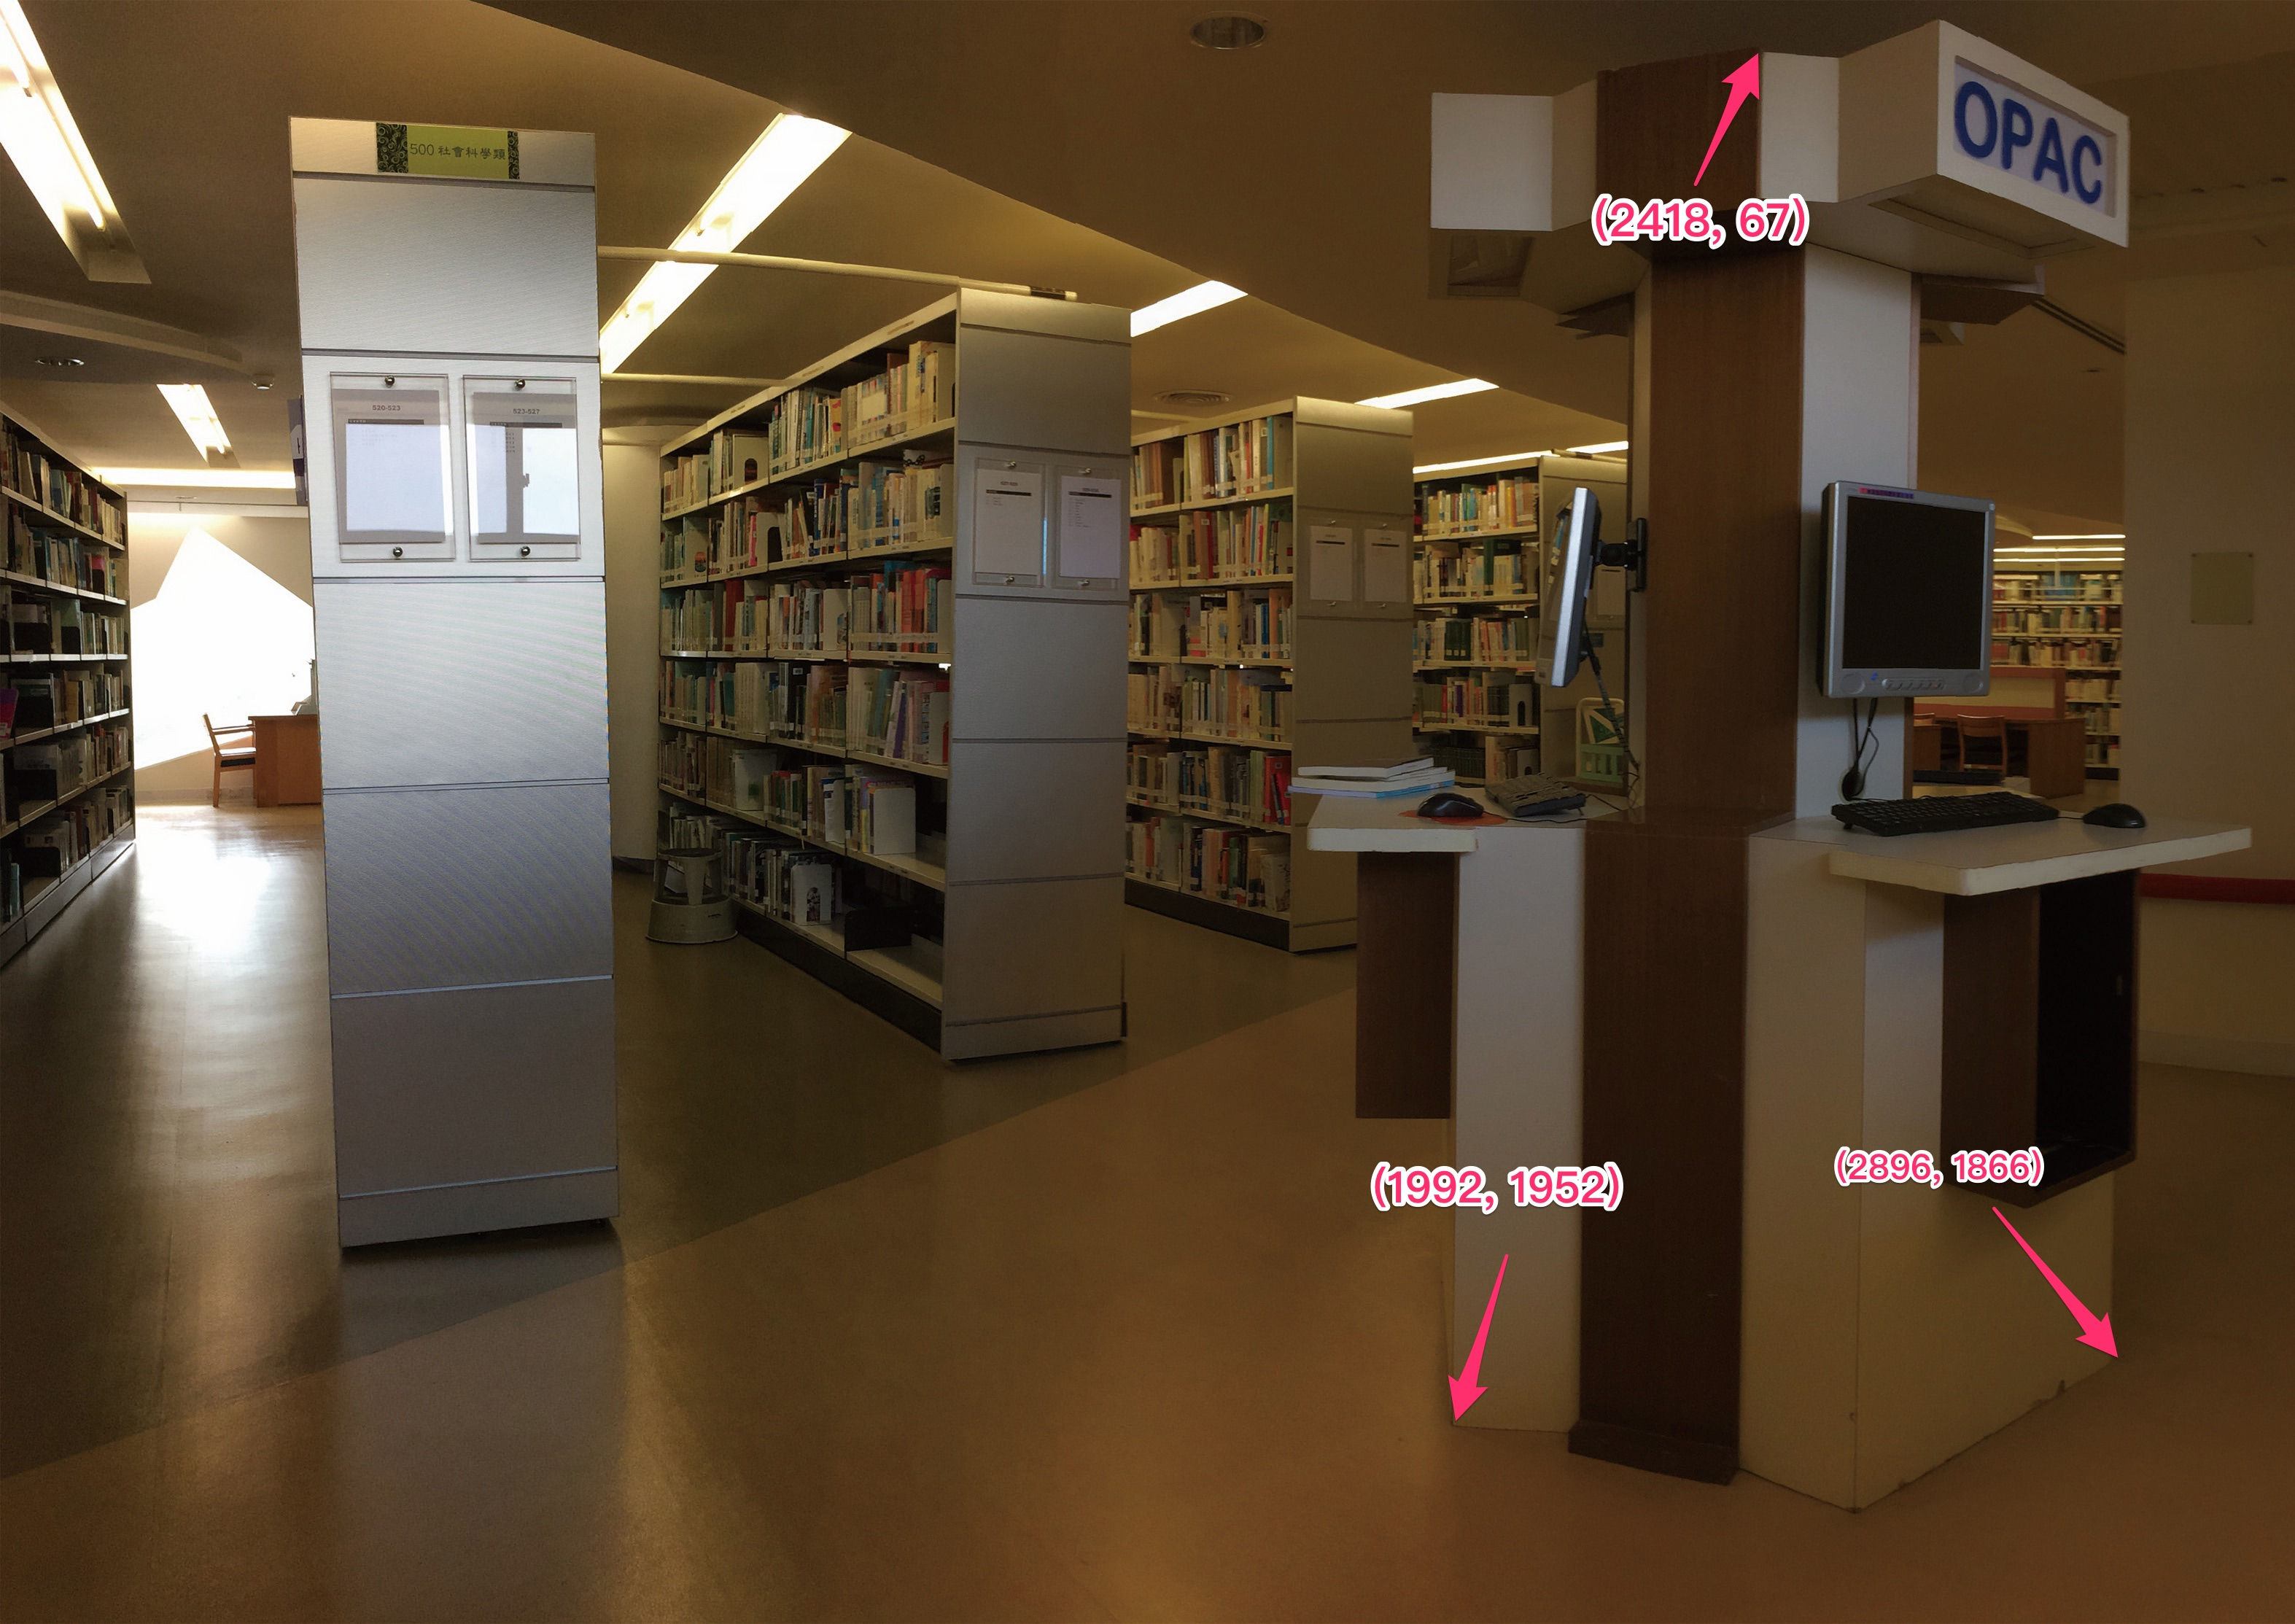
\includegraphics[width=.4\textwidth]{image/cor1.jpg}
\hspace{1cm}
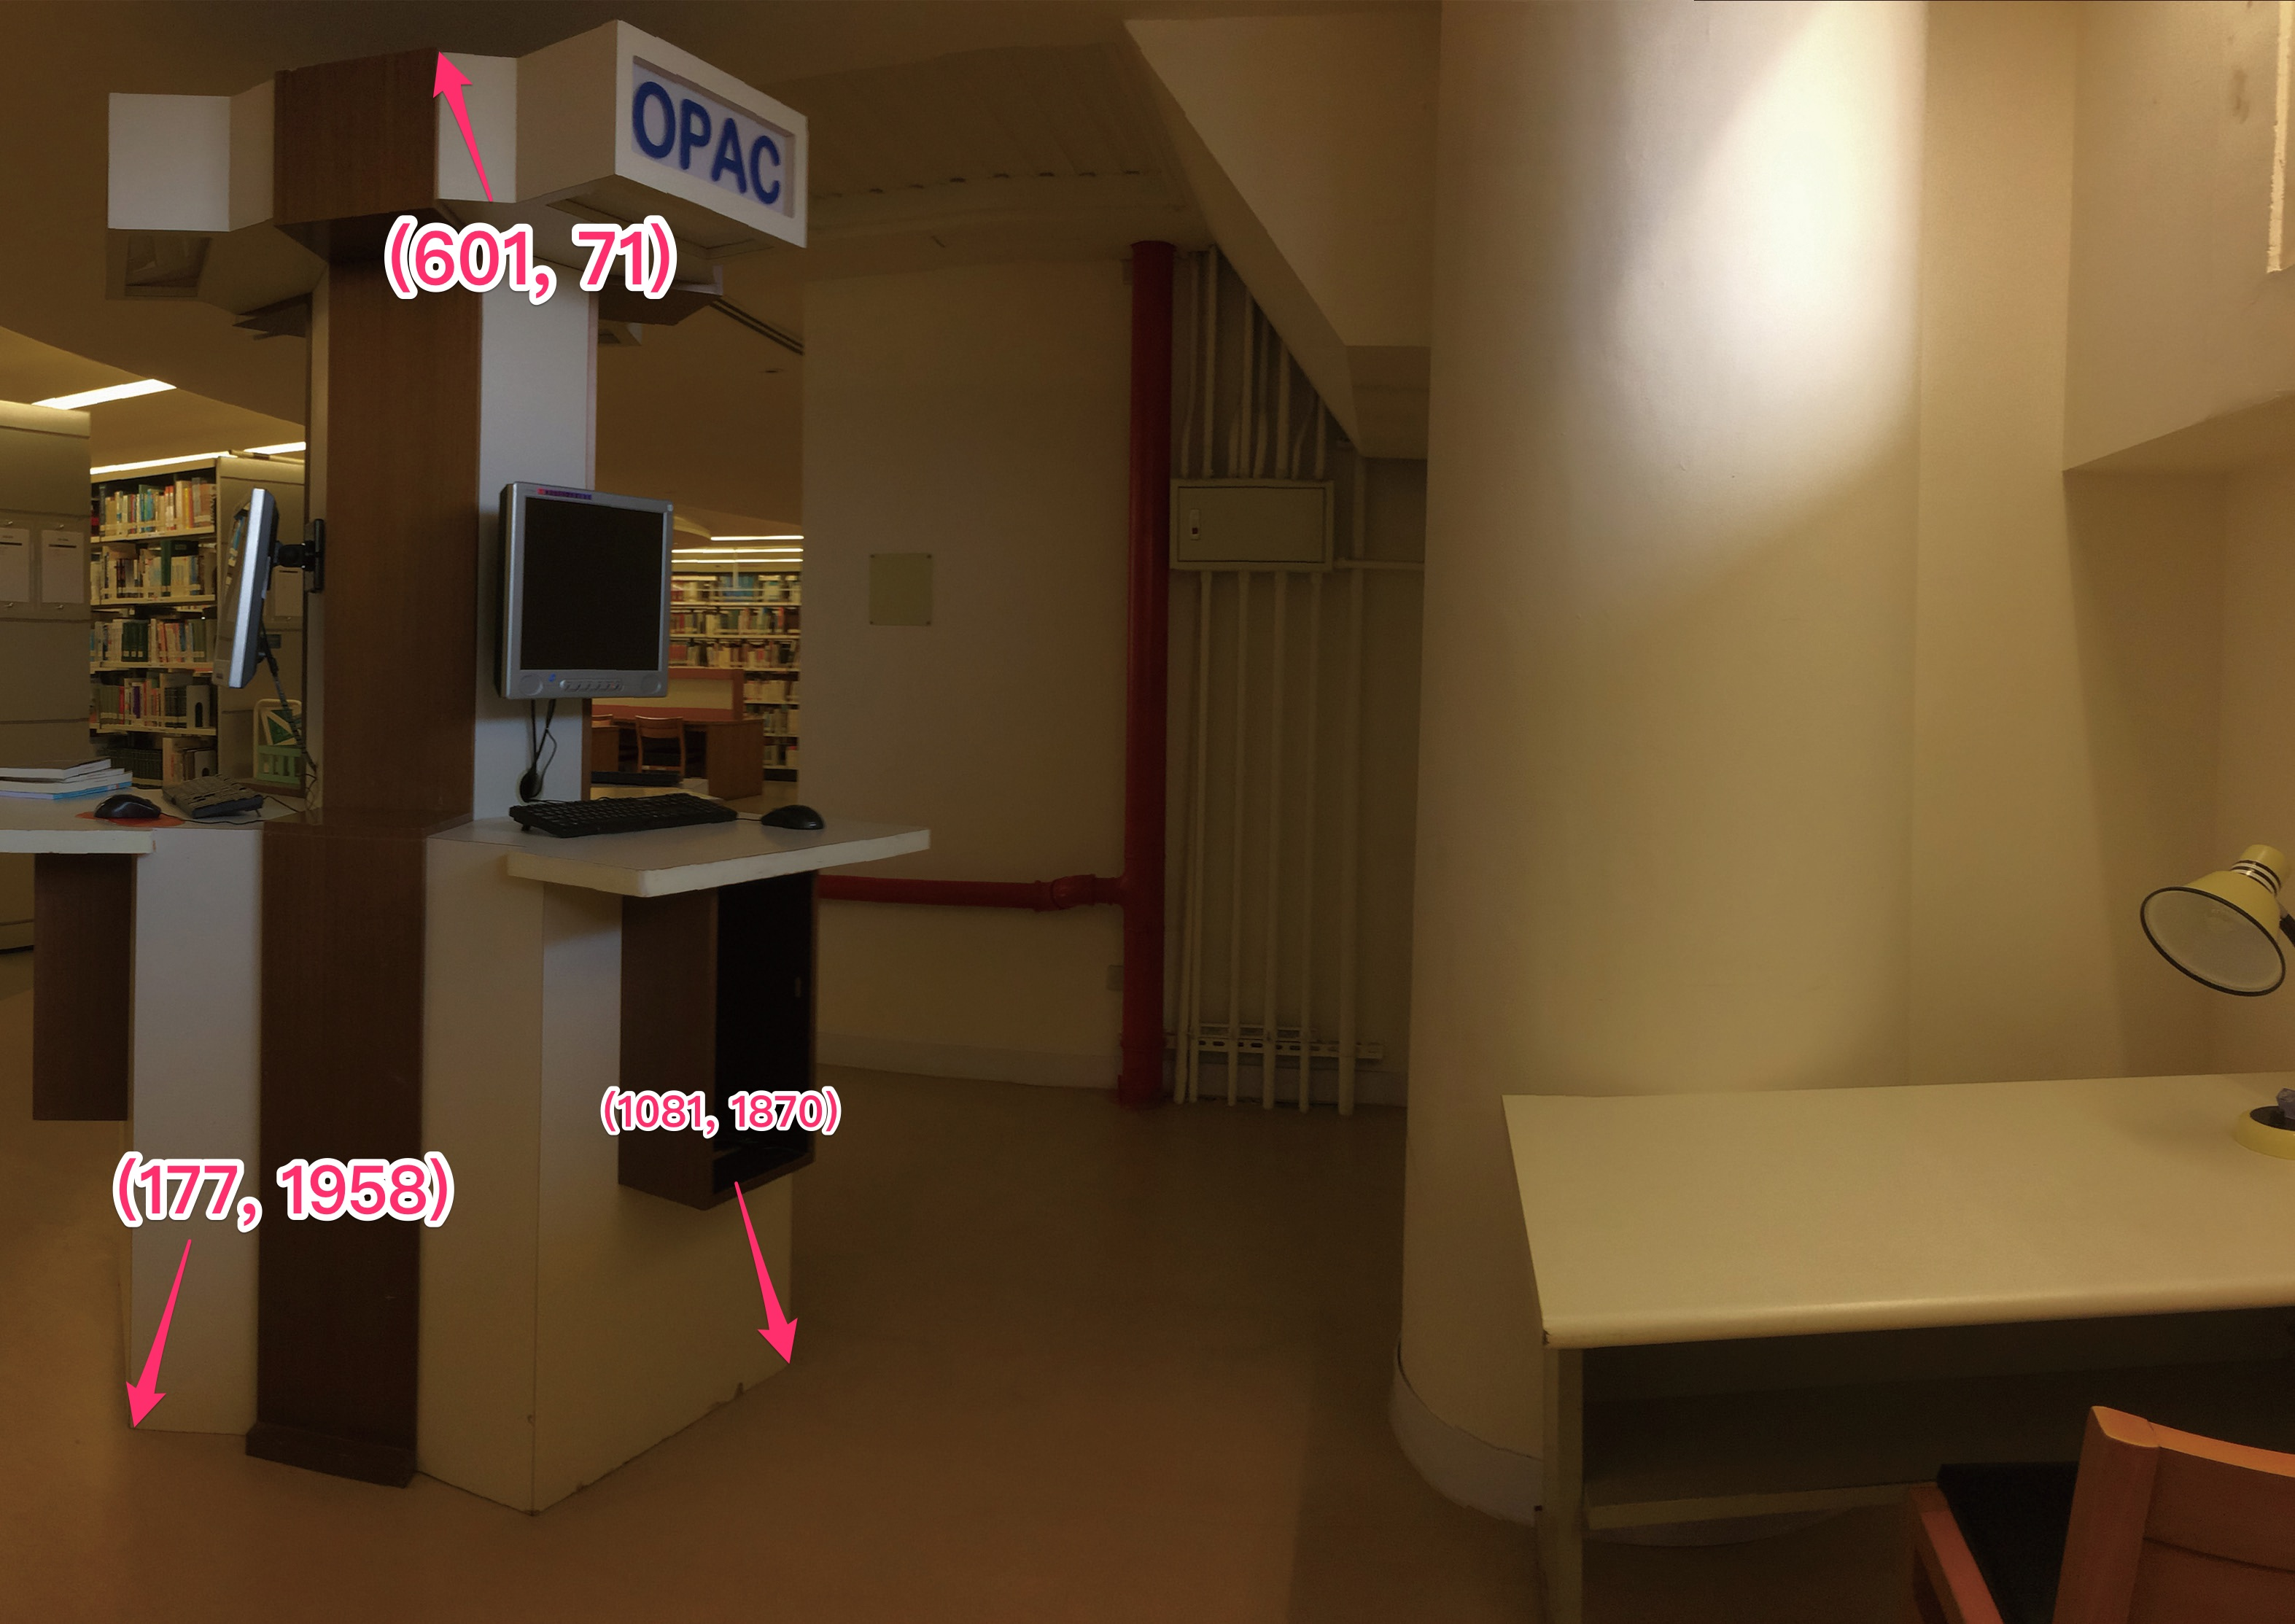
\includegraphics[width=.4\textwidth]{image/cor2.jpg}
\caption{combine pictures}%整個標籤
\label{要合併的兩張圖}%整個圖形標籤
\end{figure}
}

\newpage % 新一頁
\subsection{六參數}

{
\fontsize{14pt}{10pt} % 字型大小12pt,字行間距10pt
\selectfont % 生效
用上面兩張圖的3個座標,透過Ax=B找出六參數
\newline
\newline 矩陣
\[ % begin math mode 
\left(
\begin{array}{clr}
2418 & 67 & 1 \\ 1992 & 1952 & 1 \\ 1896 & 1866 & 1
\end{array}
\right)
\left(
\begin{array}{clr}
a \\ b \\ c
\end{array}
\right)
=
\left(
\begin{array}{clr}
601 \\ 177 \\ 1081
\end{array}
\right)
\] % end math mode

\[ % begin math mode 
\left(
\begin{array}{clr}
2418 & 67 & 1 \\ 1992 & 1952 & 1 \\ 1896 & 1866 & 1
\end{array}
\right)
\left(
\begin{array}{clr}
d \\ e \\ f
\end{array}
\right)
=
\left(
\begin{array}{clr}
71 \\ 1958 \\ 1870
\end{array}
\right)
\] % end math mode

程式碼
\begin{lstlisting}[language=Python]

# 取得六參數
def getFunctionParaOfX():
    a = np.array([[2418, 67, 1], 
    			[1992, 1952, 1], 
    			[2896, 1866, 1]])
    b = np.array([601, 177, 1081])
    x = np.linalg.solve(a, b)
    return x

def getFunctionParaOfY():
    a = np.array([[2418, 67, 1], 
    			[1992, 1952, 1], 
    			[2896, 1866, 1]])
    b = np.array([71, 1958, 1870])
    y = np.linalg.solve(a, b)
    return y
    
# 轉換座標
def getTransferCoordinate(X, Y, x, y):
    newX = X[0] * x + X[1] * y + X[2]
    newY = Y[0] * x + Y[1] * y + Y[2]
    return (newX, newY)
\end{lstlisting}
}

\newpage % 新一頁
\subsection{Bilinear Interpolation }
{
因為輸出像素對應的地方,不一定是輸入圖像某個整數像素位置,這時要用整數座標的灰度值進行推斷
\begin{figure}[ht]
\centering
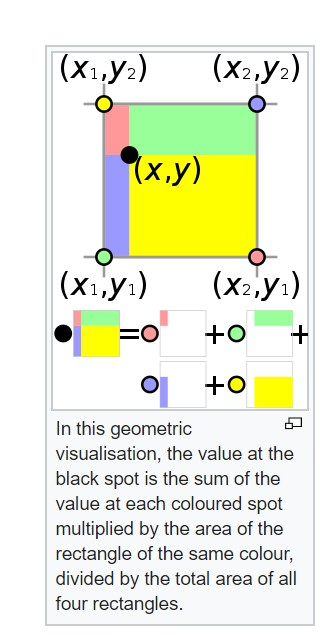
\includegraphics[width=.4\textwidth]{image/bilinear.jpg}
\caption{Bilinear}%整個標籤
\label{Bilinear}%整個圖形標籤
\end{figure}

程式碼
\begin{lstlisting}[language=Python]

# 做Bilinear Interpolate
def getBilinearInterpolate(im, x, y):
    x = np.asarray(x)
    y = np.asarray(y)

    x0 = np.floor(x).astype(int)
    x1 = x0 + 1
    y0 = np.floor(y).astype(int)
    y1 = y0 + 1

    x0 = np.clip(x0, 0, im.shape[1] - 1)
    x1 = np.clip(x1, 0, im.shape[1] - 1)
    y0 = np.clip(y0, 0, im.shape[0] - 1)
    y1 = np.clip(y1, 0, im.shape[0] - 1)

    imA = im[y0, x0]
    imB = im[y1, x0]
    imC = im[y0, x1]
    imD = im[y1, x1]

    wa = (x1 - x) * (y1 - y)
    wb = (x1 - x) * (y - y0)
    wc = (x - x0) * (y1 - y)
    wd = (x - x0) * (y - y0)

    result = wa * imA + wb * imB + wc * imC + wd * imD
    return result
\end{lstlisting}
}

\subsection{合併圖片}

{
先產生一張可以包含合併後圖片大小的圖,再用兩個for-loop跑長寬,如果座標是在照片一內,則直接輸出照片一的像素。

如果不再照片一的範圍,則透過轉換座標判斷是否在照片二的座標內,如果是,則透過Bilinear Interpolate算出該像素值,如果不是則給黑色。

程式碼
\begin{lstlisting}[language=Python]

# 處理新照片
print('start process photo')
for x in range(width):
    for y in range(height):
        if y < 2227 and x < 3147:
            newImage[y][x] = getBilinearInterpolate(im1, x, y)
        else:
            newX, newY = getTransferCoordinate(X, Y, x, y)
            if 0 <= newY < 2227 and 0 <= newX < 3147:
                newImage[y][x] = getBilinearInterpolate(im2, 
                										newX,
                										newY)
            else:
                newImage[y][x] = 0
print('process photo done')
\end{lstlisting}
}

\section{結論}

一開始拍攝兩張照片,但角度問題會造成要合併的物件大小在兩張照片是不相同,導致兩張照片合併時會有大小的落差。

所以後來改成先拍一張大圖,裁切成兩張後進行合併。
\begin{figure}[ht]
\centering
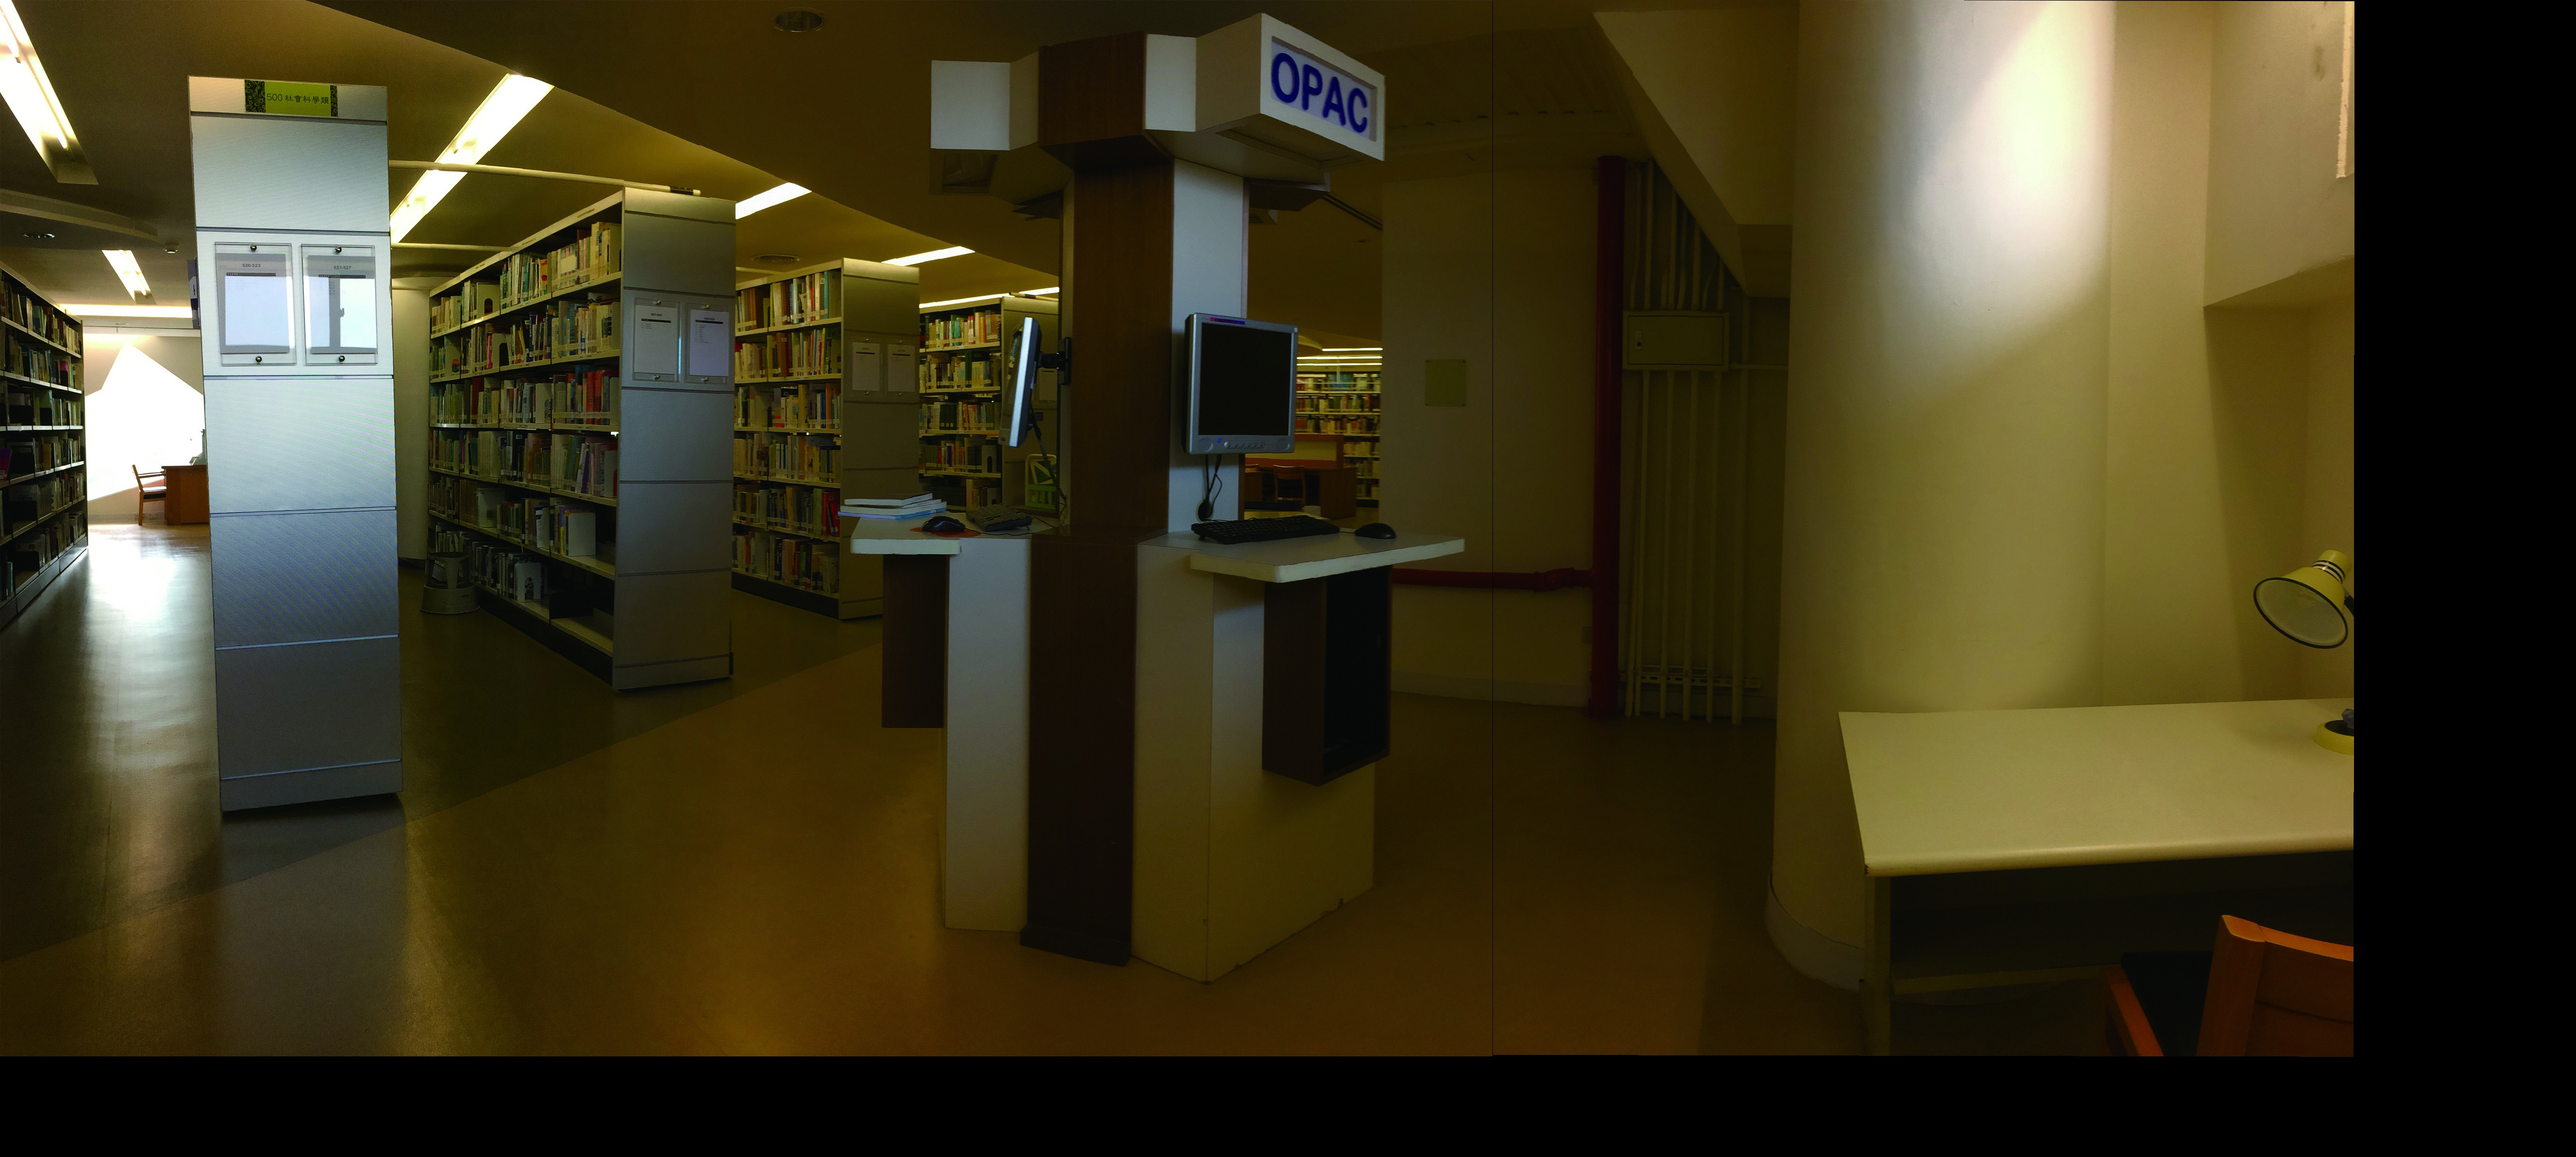
\includegraphics[width=1\textwidth]{image/combineBilinearPhoto.jpg}
\caption{合併影像}%整個標籤
\label{合併影像}%整個圖形標籤
\end{figure}
\end{document}